
\subsection{Ergebnisse}

Die Kopf-Orientierung wird auf Basis verschiedener Sensordaten bestimmt.
Die aus unterschiedlichen Kombinationen der Sensoren berechneten Orientierungen stehen als Ausgabe zur Verfügung:
\begin{itemize}
  \item Marker-Tracking
  \item Gyroskop + Beschleunigungssensor
  \item Gyroskop + Beschleunigungssensor + Magnetometer
  \item Gyroskop + Beschleunigungssensor + Magnetometer + Marker-Tracking
\end{itemize}

Durch Einsatz des \ac{ROS}-Frameworks und durchgängige Verwendung des Transformationsbaums (vgl. Abs. \ref{headracking_markerfusion_subsubsec}) ist dabei das Referenz-Koordinatensystem frei wählbar.
In der Visualisierung können die gewünschten Berechnungsergebnisse vom Benutzer ausgewählt werden, s. Abb. \ref{fig:kopf_orientierung_rviz}.


Die Applikation konnte erfolgreich im unbewegten CoCar getestet werden.
Tests im bewegten Fahrzeug sind noch durchzuführen.


\begin{figure}
  \centering
  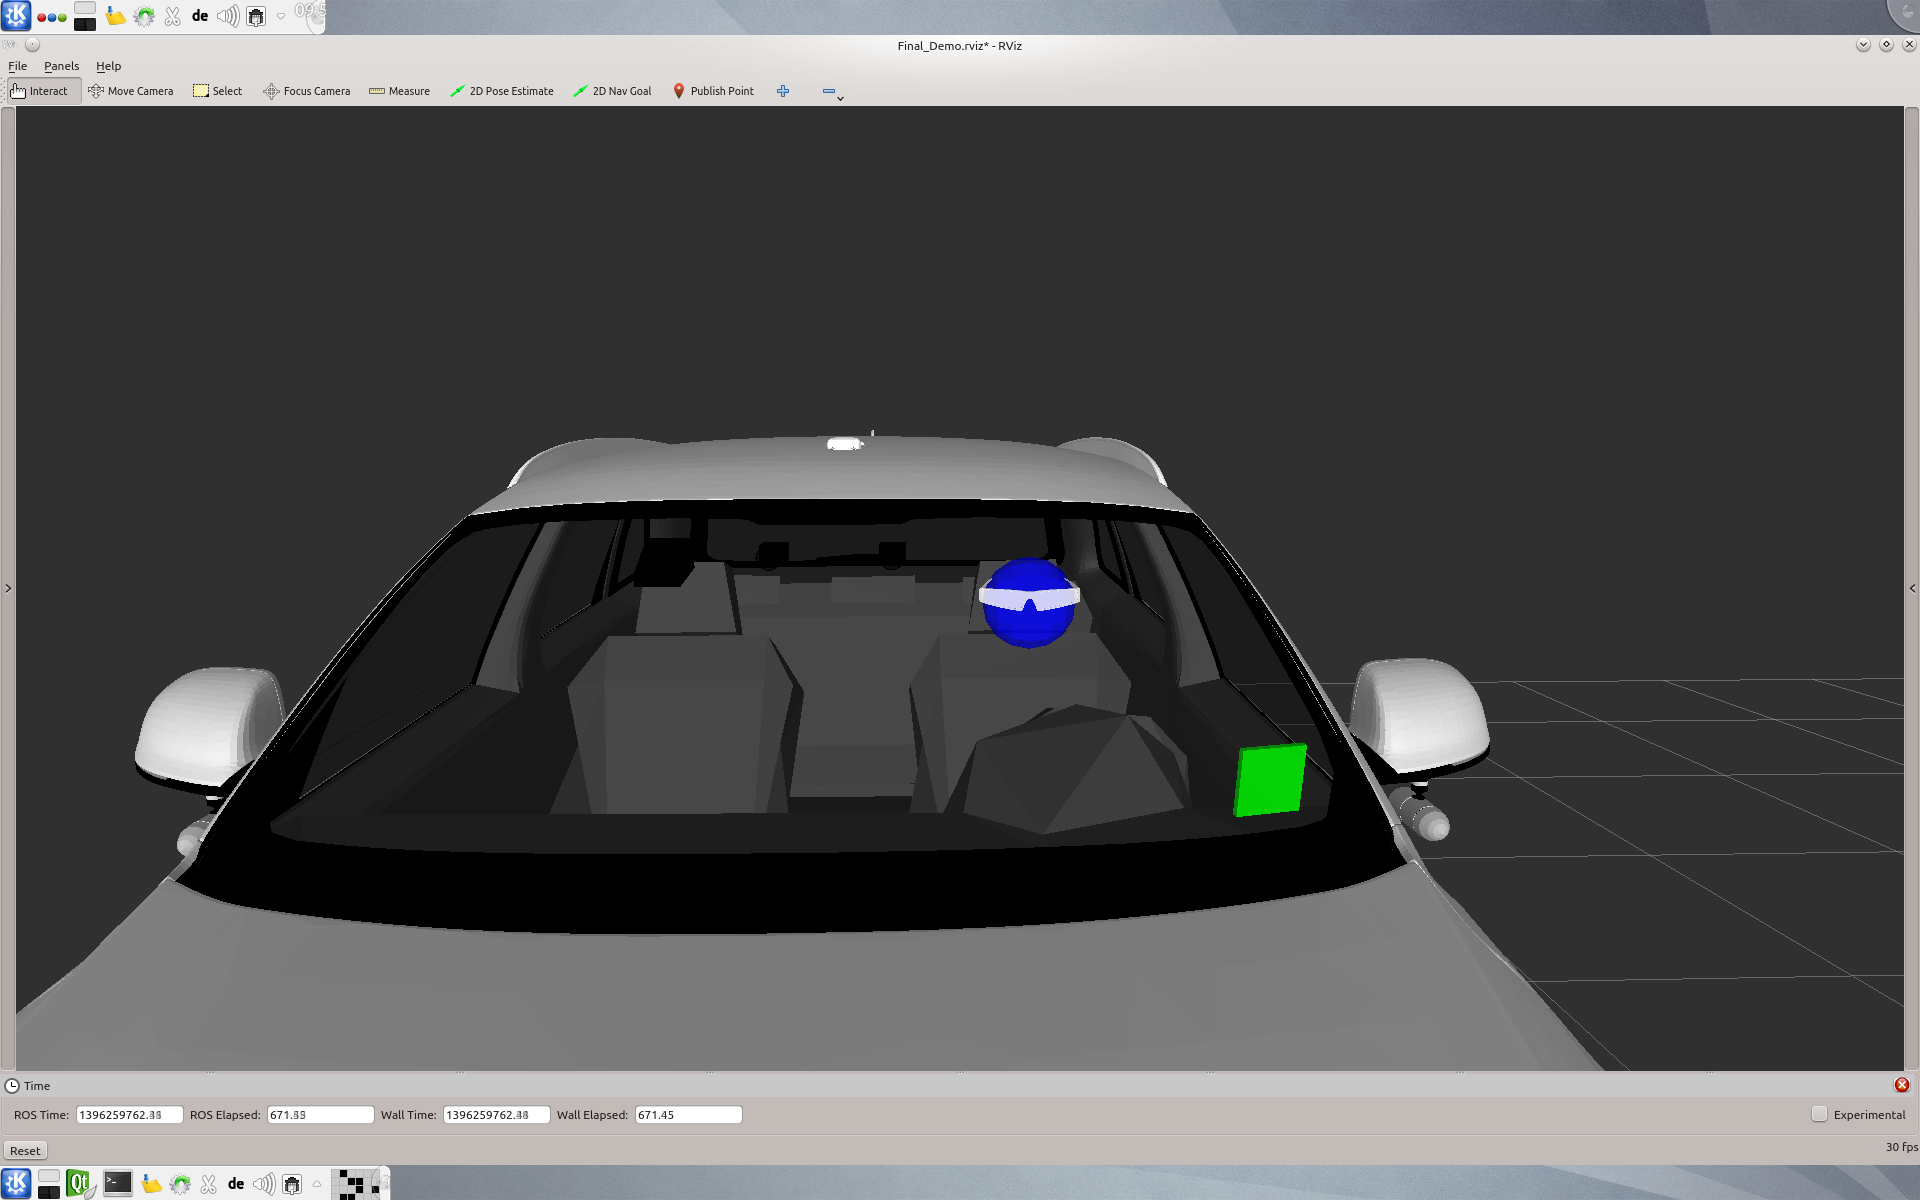
\includegraphics[width=0.4\textwidth]{Frontsicht_Kopf_Brille_RVIZ}
  \caption{Visualisierung der Kopforientierung}
  \label{fig:kopf_orientierung_rviz}
\end{figure}


\subsection{Ausblick}

Für Weiterentwicklungen des Systems bieten sich interessante Bereiche an:

Das System ist derzeit beschränkt auf die Bestimmung der Kopf-Orientierung.
Eine Erweiterung, sodass zusätzlich auch die Position des Kopfes geschätzt wird, ist sicherlich der interessanteste Ansatzpunkt.
Dazu ist eine Integration der Orientierungsdaten über die Zeit nötig.
Da von der in Abs. \ref{headtracking_markertracking_subsubsec} beschriebenen ALVAR-Bibliothek auch --bisher nicht verwendete-- Positionsinformationen geliefert werden, kann voraussichtlich die Stützung durch Kameradaten zu großen Teilen unverändert übernommen werden.

Außerdem bietet ALVAR eine Bundle-Funktionalität, die bisher noch nicht eingesetzt wird.
Damit können im Innenraum des Autos weitere Marker angebracht werden, sodass bei nahezu beliebiger Blickrichtung des Fahrers immer ein Marker im Kamerabild zu erkennen ist.
Die Korrektur der \ac{IMU}-Daten durch Kameradaten wäre damit nicht mehr auf eine Blickrichtung in Fahrtrichtung beschränkt.

Möglich ist auch eine weitere Untersuchung des in Abs. \ref{headtracking_facetracking_subsubsec} beschriebenen Face-Trackings.
Hier ist die Erstellung einer neuen Gesichts-Maske --mit \ac{AR}-Brille-- ein vielversprechender Ansatz. \todo{Ist das so? Es gibt doch einige Argumente dagegen.}

Ein Ausbau der Hardware-Kompatibilität auf weitere Brillen-Modelle wie beispielsweise \emph{Google Glass, Oculus Rift} \oae erscheint ebenfalls interessant.


